\subsection{Definició i llei de grup}

\begin{definition}
 Una \emph{corba el·líptica} sobre un cos $K$ és una equació de la forma
 \[
 E\colon y^2 + a_1 xy + a_3 y = x^3 + a_2 x^2 + a_4 x + a_6,
 \]
 on $a_1, a_2, a_3, a_4, a_6\in K$ són tals que
 \[
 \Delta_E = -b_2^2b_8-8b_4^3-27b_6^2+9b_2b_4b_6 \neq 0,
 \]
 amb
 \begin{align*}
 b_2&=a_1^2+4a_2,\\
 b_4&=2a_4+a_1a_3,\\
 b_6&=a_3^2+4a_6, \text{ i}\\
 b_8&=a_1^2a_6+4a_2a_6-a_1a_3a_4+a_2a_3^2-a_4^2.
 \end{align*}
\end{definition}
\begin{remark}
 Si la característica de $K$ és diferent de $2$, aleshores es pot fer un canvi afí de variables que permet escriure $E$ de forma
 \[
 E\colon y^2 = x^3 + ax +b, \quad a,b\in K.
 \]
 En aquest cas, el discriminant $\Delta_E$ té una expressió més senzilla:
\[
\Delta_E = -16(4a^3+27b^2).
\]
\end{remark}

Podem pensar una corba el·líptica $E$ com un cert subconjunt de $\mathbb{P}^2$. En aquest cas cal considerar l'equació homogènia ($x = X/Z$, $y=Y/Z$)
\[
E\colon Y^2Z + a_1 XYZ + a_3 YZ^2 = X^3 + a_2 X^2Z + a_4 XZ^2 + a_6 Z^3.
\]
Quan $Z=0$, obtenim com a solució el punt projectiu $\calO=(0:1:0)$, que anomenarem \emph{punt a l'infinit} d'$E$.

Donat un cos $L\supseteq K$, el conjunt de \emph{punts definits a $L$} és
\[
E(L) = \{(x,y)\in L\times L ~|~ y^2 + a_1xy + a_3 y = x^3 + a_2x^2 + a_4 x + a_6\}\cup \{\calO\}.
\]

La importància de les corbes el·líptiques en la teoria de nombres prové del fet que el conjunt de punts $E(L)$ ve dotat d'una estructura de grup abelià. Ens serà útil el següent lema geomètric:

\begin{lemma}
Tota recta interseca $E$ en tres punts, si els comptem amb multiplicitat.

A més, si dos d'aquests punts tenen coordenades a una extensió $L$, també les hi té el tercer punt.
\end{lemma}

\begin{proof}
Considerem una recta genèrica a $\P^2$, donada per l'equació
\[
\alpha X+\beta Y+\gamma Z=0, \quad \alpha,\beta,\gamma\in L.
\]
Si $\alpha=\beta=0$, aleshores es tracta de la recta a l'infinit, que interseca de manera triple amb $\calO$ com podem comprovar fàcilment.

Suposem doncs que $\alpha\neq 0$ o $\beta\neq 0$, i per tant podem treballar amb la forma no-homogènia
\[
\alpha x + \beta y + \gamma = 0.
\]
Si $\alpha \neq 0$, aleshores substituint $x = \frac{-1}{\alpha} (\gamma + \beta y)$ a l'equació d'$E$ obtenim un polinomi en $y$ de grau $3$, i per tant $3$ solucions. També, si $\beta\neq 0$, substituint $y=\frac{-1}{\beta}(\gamma + \alpha x)$ s'obté un polinomi en $x$ de grau $3$ i, per tant les tres solucions.

Suposem que dos dels punts d'intersecció tenen coordenades a $L$. Notem que, per veure que un punt té coordenades a $L$ només cal veure que o bé la seva coordenada $x$ o bé la $y$ és de $L$, ja que l'altra coordenada també ho serà fent servir l'equació de la recta. En els polinomis anteriors, que estan definits a $K$ (en $x$ o en $y$) el producte de les tres arrels és el terme constant i, per tant, és de $K\subseteq L$. Si dues de les arrels són d'$L$, aleshores la tercera també ho és.

\end{proof}


\begin{figure}[ht]
\includegraphics[page=3,width=.5\textwidth]{addingpoints.pdf}
\includegraphics[page=3,width=.5\textwidth]{doublingpoints.pdf}
\caption{Suma de dos punts a $E$}
\end{figure}

Donats dos punts $P,Q \in E(K)$, considerem la recta que $\ell_{P,Q}$ que passa per $P$ i $Q$ (en cas que $P=Q$, aleshores $\ell_{P,P}$ serà la recta tangent a $E$ que passa per $P$).

La recta $\ell_{P,Q}$ interseca en un altre punt $R\in E(K)$. Finalment, definim $P+Q$ com el tercer punt d'intersecció de la recta $\ell_{R,\calO}$.

Òbviament aquesta operació és commutativa, i és fàcil veure que el punt de l'infinit $\calO$ és l'element neutre.

Definim $-P$ com el tercer punt d'intersecció de la recta $\ell_{\calO, P}$. Per definició, $\ell_{P,-P} = \ell_{\calO, P}$, i per tant el punt $R$ és justament $\calO$. Ara, si prenem la recta tangent a $E$ que passa per $\calO$, obtenim la recta de l'infinit $\{ z=0\}$, que talla $E$ només a $\calO$ (intersecció triple). Per tant, concloem que $P+(-P)=\calO$.

L'associativitat d'aquesta operació no es veu tan trivialment, i en deixem la demostració per més endavant. Així, el conjunt de punts $K$-definits d'$E$ adquireix una estructura addicional: és un grup abelià.

\subsubsection{La llei de grup en coordenades}
Donats punts $P_1=(x_1,y_1)$ i $P_2=(x_2,y_2)$ d'$E$, volem calcular $P_3=(x_3,y_3)=P_1+P_2$. Fixem-nos que, si $P_1=\calO$ o $P_2=\calO$ aleshores el resultat és clar. També si $P_2=-P_1$. Per tant, suposarem que aquest no és el cas. Per simplificar les fórmules, treballarem amb el model
\[
y^2=x^3+a_2x^2+a_4x + a_6.
\]
En aquest cas, fixem-nos que si $P=(x,y)$ aleshores $-P=(x,-y)$.

La recta $\ell_{P_1,P_2}$ té equació $y = \lambda (x-x_1) + y_1$, on
\[
\lambda=\begin{cases}
\frac{y_2-y_1}{x_2-x_1}&\text{si } P_1\neq P_2,\\
\frac{3x^2+2a_2x + a_4}{2y}&\text{si } P_1=P_2.
\end{cases}
\]
Substituint-ho a l'equació d'$E$, obtenim un polinomi de grau $3$ en $x$, del qual ens fixarem en el terme de grau $2$, que és $a_2-\lambda^2$. Aquest terme es correspon a $-(x_1+x_2+x_3)$ i, per tant, podem aïllar
\[
x_3 = \lambda^2-a_2-x_1-x_2.
\]
La coordenada $y$ de $P_3$ és l'oposat del punt d'intersecció que acabem de calcular. Per tant, obtenim:
\[
y_3 = \lambda (x_1-x_3)-y_1.
\]

Aquestes formules ens permeten verificar l'associativitat de la suma ajudant-nos de \texttt{Sage}.

\begin{proposition}
\begin{enumerate}
    \item Si $P,Q,R$ satisfan que els elements
    \[
    \{P,-P,Q,-Q,R,-R,P+Q,-(P+Q),(Q+R),-(Q+R),\calO\}
    \]
    són tots ells diferents, aleshores
    $P+(Q+R)=(P+Q)+R$.
    \item Si $P,Q$ satisfà que els elements $\{P, -P, 2P, -2P, Q, \calO\}$ són tots ells diferents, aleshores
    \[
    2P+Q = P+(P+Q).
    \]
    \item Si $P\in E(K)$, aleshores
    \[
    2(P+Q) = P + (Q + (P + Q)).
    \]
\end{enumerate}
\end{proposition}
\begin{proof}
 El següent codi en \texttt{Sage} verifica les equacions algebraiques que es corresponen a cada igualtat.

\begin{python}
S.<a1, a2, a3, a4,a6, x1, x2, x3,y1,y2,y3> = PolynomialRing(QQ, 11)
I = S.ideal([y1^2 + a1*x1*y1 + a3*y1 -(x1^3 + a2*x1^2 + a4*x1 + a6), \
             y2^2 + a1*x2*y2 + a3*y2 - (x2^3 + a2*x2^2 + a4*x2 + a6), \
             y3^2 + a1*x3*y3 + a3*y3 -(x3^3 + a2*x3^2 + a4*x3 + a6)])
P, Q, R = (x1,y1), (x2,y2), (x3,y3)

def add(P,Q):
    s1 = (Q[1]-P[1]) / (Q[0]-P[0])
    xPQ = s1^2 + a1 *s1 - a2 - P[0] - Q[0]
    yPQ = -a1 * xPQ -a3 - P[1] + s1*(P[0] - xPQ)
    return (xPQ, yPQ)

def double(P):
    s1 = (3*P[0]**2 + 2*a2 *P[0] -a1*P[1]+ a4) / (2 * P[1] + a1*P[0] + a3)
    xPQ = s1^2 + s1*a1 - a2 - 2*P[0]
    yPQ = -a1 * xPQ -a3 - P[1] + s1*(P[0] - xPQ)
    return (xPQ, yPQ)

A = add( add(P, Q), R )
B = add(P, add(Q, R) )
print( (A[0] - B[0]).numerator() in I and (A[1] - B[1]).numerator() in I )

A = add(double(P),Q)
B = add(P,add(P,Q))
print( (A[0] - B[0]).numerator() in I and (A[1] - B[1]).numerator() in I )

A = double(add(P,Q))
B = add(P,add(Q,add(P,Q)))
print( (A[0] - B[0]).numerator() in I and (A[1] - B[1]).numerator() in I )
\end{python}
\end{proof}

\begin{lemma}
Per a qualssevol punts $P$, $Q$ i $R$ de la corba $E$, es satisfà:
 \begin{enumerate}
     \item $(P+Q)-Q = P$.
     \item $P+R = Q+R \iff P = Q$.
     \item $2P + Q = P+(P+Q)$.
 \end{enumerate}
\end{lemma}
\begin{proof}
 La primera afirmació es comprova amb la definició de suma, fent servir que la recta simètrica a $\ell_{P,Q}$ és la recta $\ell_{P+Q,-Q}$.
 
 La segona afirmació segueix de la primera: si $P+R=Q+R$, aleshores $P = (P+R)-R = (Q+R) -R = Q$.
 
 Finalment, per comprovar l'última afirmació primer cal veure-la quan $Q$ és $\calO$ o $\pm P$, i en aquests casos és fàcil comprovar-ho pel què hem vist fins ara. Si $2P=\calO$ també és fàcil, així com quan $Q=-2P$. El cas $Q=2P$ i el cas general són precisament els que s'han comprovat amb \texttt{Sage}.
\end{proof}
\begin{corollary}
Per a qualssevol punts $P$ i $Q$ d'$E$, es satisfà:
 \begin{enumerate}
     \item $((P+Q)+P)+Q = 2(P+Q)$.
     \item $P+(Q-(P+Q))=\calO$.
 \end{enumerate}
\end{corollary}

Amb aquests resultats, podem demostrar ja l'associativitat de la suma.
\begin{theorem}
La llei de grup definida anteriorment és associativa. Per tant, defineix un grup abelià.
\end{theorem}
\begin{proof}
 Els casos on $\calO\in\{P,Q,R\}$ són obvis. Els casos especials queden coberts amb el lema i corol·lari anteriors, i el cas general s'ha comprovat amb \texttt{Sage}.
\end{proof}
 \subsection{Punts de torsió, punts racionals}
 Donada una corba el·líptica $E$ definida sobre un cos $K$, definim el subgrup de torsió com
 \[
 E(K)_\tors = \{P\in E(K) ~|~ nP=\calO,\text{ per algun } n\geq 1\}.
 \]
 També definim, per cada $n\geq 1$, el subgrup
 \[
 E[n](K) = \{P\in E(K) ~|~ nP=\calO\},
 \]
 de manera que
 \[
 E(K)_\tors = \bigcup_{n\geq 1} E[n](K).
 \]
 Més endavant també ens convindrà escriure $E[n] = E[n](\bar K)$.
 
 El següent resultat, que no demostrarem aquí, ens dona una manera de trobar tots els punts de torsió d'una corba el·líptica definida sobre $\Q$.
 \begin{theorem}[Nagell--Lutz (1935, 1937)]
 Sigui $E$ una corba el·líptica amb equació
 \[
 y^2=x^3+ax^2+bx+c,\quad a,b,c\in\Z.
 \]
 Si $P=(x,y)$ pertany a $E(\Q)_\tors$, aleshores:
 \begin{enumerate}
     \item $x,y\in\Z$, i
     \item $y=0$ o $y^2 \mid -4a^3c+a^2b^2+18abc-4b^3-27c^2=\Delta_E/16$.
 \end{enumerate}
 \end{theorem}
\begin{remark}
Fent un canvi de variables de la forma $(x',y') = (u^2 x +r , u^3 y)$, amb un $u\in\Q^\times$ i $r\in \Q$ adequats,  es pot aconseguir sempre que $a,b,c$ siguin enters.
\end{remark}

\begin{remark}
Observem que el recíproc no és cert. Per exemple, el punt $P=(1,1)$ de la corba $y^2=x^3-16x+16$ té ordre infinit. De fet, si $P$ fos torsió aleshores $2P$ també ho seria, però $2P=(161/4,2033/8)$, que no té coordenades enteres.
\end{remark}
\begin{example}
Considerem la corba el·líptica
\[
E\colon y^2=x^3-15x+22
\]
Calculem $\Delta_E /16= 6912/16 = 2^4\cdot 3^3$. Per tant, els possibles valors de $y$ tals que $y^2$ divideixi $\Delta_E/16$ són, llevat de signe, $1, 2, 4, 3, 6, 12$. Comprovant totes les possibilitats, obtenim $\{(-1,\pm 6), (3,\pm 2)\}$. Comprovem que els múltiples de $P=(-1,6)$ són

\begin{center}
  \begin{tabular}{llllll}
\toprule
     $P$ & $2P$ & $3P$ & $4P$ & $5P$ & $6P$ \\
\midrule
$(-1,6)$&$(3,-2)$&$(2,0)$&$(3,2)$&$(-1,-6)$&$\mathcal{O}_E$\\
\bottomrule
\end{tabular}
\end{center}

Per altra banda, les arrels racionals de $x^3-15x+22$ han de ser divisors de $22$, és a dir que $x$ hauria de ser, llevat de signe $1,2, 11, 22$. Comprovant totes les possibilitats, obtenim el punt de $2$-torsió $(2, 0)$ que ja havíem vist abans.

Per tant, deduïm que $E(\Q)_\text{tors} \cong \Z/6\Z$, generat per $(-1,6)$.
\end{example}

Bastants anys més tard, Barry Mazur va demostrar un teorema molt més difícil, que ens diu l'estructura d'$E(\Q)_\tors$ de manera precisa.
\begin{theorem}[Mazur, 1978]
Sigui $E$ una corba el·líptica definida a $\Q$. Aleshores
\[
E(\Q)_\tors\cong\begin{cases}
\Z/N\Z & 1 \leq N \leq 10,\text{ o } N=12,\\
\Z/2\Z\oplus \Z/2N\Z & 1\leq N \leq 4.
\end{cases}
\]
A més, tots els $15$ possibles subgrups de torsió es donen.
\end{theorem}

El següent teorema fou demostrat per Louis Mordell el 1922, i dedicarem unes quantes pàgines a la seva demostració.

\begin{theorem}[Mordell, 1922]
El grup $E(\Q)$ està generat per un nombre finit de punts.
\end{theorem}

Gràcies al teorema de classificació dels grups abelians finitament generats, en deduïm que
\[
E(\Q) = E(\Q)_\tors \oplus \Z^r,\quad r\geq 0.
\]
L'enter $r$ s'anomena el \emph{rang de Mordell--Weil} d'$E(\Q)$, i avui en dia no hi ha cap algoritme\footnote{Per algoritme volem dir un programa d'ordinador el qual podem garantir que acabi en temps finit.} per calcular-lo, encara que hi ha mètodes que funcionen bastant bé.



\subsubsection{Altures}
Volem definir l'``altura'' d'un racional, de manera que hi hagi finits racionals d'altura fixada.
\begin{definition}
L'\emph{altura} d'un racional $\frac{a}{b}\in\Q$ és
\[
h(a/b) = \log \max\{|a|,|b|\},\quad\text{ si } \gcd(a,b)=1.
\]
Si $P=(x,y)\in E(\Q)$, l'\emph{altura} de $P$ és $h(P)=h(x)$, l'altura de la seva coordenada-$x$. També escriurem $h(\calO)=0$.
\end{definition}

\begin{remark}
Per cada $M>0$, el conjunt $E(\Q)_{\leq M} = \{ P\in E(\Q) ~|~ h(P) \leq M\}$ és finit.
\end{remark}

\begin{lemma}
Sigui $Q_0\in E(\Q)$. Hi ha una constant $C(Q_0)$ tal que
\[
h(P+Q_0)\leq 2h(P) + C(Q_0), \quad \forall P\in E(\Q).
\]
\end{lemma}
\begin{lemma}
Hi ha una constant $C$ tal que
\[
h(2P)\geq 4h(P) - C,\quad \forall P\in E(\Q).
\]
\end{lemma}

\begin{theorem}
Si $E(\Q)/2E(\Q)$ és finit, aleshores $E(\Q)$ és finitament generat.
\end{theorem}
\begin{proof}
Siguin $Q_1,\ldots, Q_t$ representants del quocient $E(\Q)/2E(\Q)$.
Per tant, donat $P=P_0\in E(\Q)$, podem escriure $P_0 = Q_{i_0} + 2P_1$, amb $P_1\in E(\Q)$. Repetint l'argument amb $P_1$, podem escriure $P_1 = Q_{i_1} + 2P_2$. Per tant,
\[
P = Q_{i_0} + 2P_1 = Q_{i_0} + 2Q_{i_1} + 4P_2.
\]
Després de $n$ iteracions d'aquest argument, obtenim
\[
P = Q_{i_0} + 2Q_{i_1} + 4Q_{i_2}+\cdots +2^{n-1} Q_{i_{n-1}} + 2^{n}P_n
\]
Calculem ara l'altura de $P_j$, per cada $j$. Si escrivim $\bar C = \max\{ C(Q_1),\ldots C(Q_t)\}$, tenim
\[
h(P - Q_i) \leq 2h(P) + C(Q_i)\leq 2h(P) + \bar C.
\]
Aleshores,
\[
4h(P_j)\leq h(2P_j) + C = h(P_{j-1} - Q_{i_{j-1}}) + C\leq 2h(P_{j-1}) + \bar C + C.
\]
Per tant, escrivint $M=\bar C + C$, tenim
\[
h(P_j)\leq \frac{1}{2} h(P_{j-1}) + \frac{M}{4} = \frac{3}{4} h(P_{j-1}) - \frac 14\left(h(P_{j-1}) - M\right).
\]
D'aquí en traiem:
\[
\text{Si } h(P_{j-1})\geq M,\text{ aleshores } h(P_j)\leq \frac 34 h(P_{j-1}).
\]
Per tant, si observem la successió de punts $P_0, P_1, P_2, \ldots$, si tenen altura més gran que $M$, aleshores la seva altura cada vegada es fa més petita (tendint a zero). Aleshores hi ha algun índex $n$ tal que $P_n\in E(\Q)_{\leq M} = \{ P\in E(\Q) ~|~ h(P) \leq M\}$.

Concloem que tot punt $P\in E(\Q)$ es pot escriure com a combinació lineal entera dels punts $Q_1,\ldots Q_t$ i dels finits punts de $E(\Q)_{\leq M}$.
\end{proof}

 \subsubsection{La versió dèbil del teorema de Mordell}
 Ens hem reduït a demostrar el següent resultat.
 \begin{theorem}[Mordell--Weil dèbil]
 El quocient $E(\Q)/2E(\Q)$ és finit.
 \end{theorem}
 \begin{remark}
 De fet, el teorema de Mordell--Weil afirma que, donat un cos de nombres $K$ i un enter $m\geq 2$, el quocient $E(K)/mE(K)$ és finit. Encara que la idea de la demostració és la mateixa, alguns dels ingredients que apareixen en aquest cas més general fan servir eines més avançades que preferim no introduir.
 \end{remark}
 
 Primer ens cal estudiar el grup de $2$-torsió $E[2]$. Fixem-nos que $2P=\calO$ si i només si $P=\calO$ o $P=(x,0)$. Per tant, els punts no trivials de $2$-torsió es corresponen amb les arrels de $x^3+ax+b$. Així, $E[2]$ té ordre $4$. Com que és un grup d'exponent $2$, en deduïm que
 \[
 E[2] \cong \Z/2\Z \oplus \Z/2\Z.
 \]
 En general, $E[m]\cong \Z/m\Z\oplus \Z/m\Z$ per a tot $m$. Tot i que no ho veurem aquí, sí que és fàcil demostrar que:
 
\begin{proposition}
Per a tot $m\geq 2$, el grup $E[m]=E[m](\bar K)$ és finit.
\end{proposition}
\begin{proof}
Podem suposar (ja que $K$ és de característica zero) que $E$ té per equació $y^2=x^3+Ax+B$ amb $A,B\in K$. Fent inducció en $m$, és fàcil veure que l'aplicació ``multiplicar per $m$'' s'escriu, en coordenades,
$(x,y)\mapsto \left(\frac{u(x)}{v(x)},\frac{s(x)}{t(x)}y\right)$ per certs polinomis $u,v,s,t\in K[x]$.

Per tant, $m(x,y) =\calO$ si, i només si, $v(x)=0$ (si i només si $t(x)=0$). Com que $v(x)$ té un nombre finit d'arrels, hi ha un nombre finit de possibles coordenades-$x$ pels punts d'$E[m]$ i d'aquí en deduïm el resultat.
\end{proof}

Per cada punt $P\in E(K)$, escollim $Q=(x,y)\in E(\bar K)$ tal que $mQ=P$, i definim $L_P=K(x,y)$ com la mínima extensió de $K$ que conté les coordenades $x$ i $y$ de $Q$. Definim també $L$ com la clausura normal de la composició de totes les extensions $L_P$.

Considerem l'aplicació
\[
\phi_P\colon \Gal(L/K)\to E[m],\quad \phi_P(\sigma) = \sigma(Q)-Q.
\]
Observem que
\[
m(\sigma(Q)-Q) = m\sigma(Q)-mQ= \sigma(mQ)- mQ = \sigma(P)-P = \calO,
\]
i per tant $\phi_P(\sigma)\in E[m]$.

Ens agradaria veure que l'aplicació $\phi_P$ no depèn del punt $Q$ triat. Per això, ens caldrà suposar que:

\textbf{Hipòtesi: } $E[m]\subseteq E(K)$.

Si $R$ és una altre punt tal que $mR=P$, aleshores es té $m(Q-R)=P-P=\calO$ i, per tant, $Q-R\in E[m]$. Com que $E[m]\subseteq E(K)$, aleshores
\[
(\sigma(Q)-Q) - (\sigma(R)-R) = \sigma(Q-R)-(Q-R) = (Q-R)-(Q-R)=\calO.
\]
Per tant, $\phi_P$ només depèn de $P$, i no pas del punt $Q\in E(L)$ tal que $mQ=P$.

\begin{remark}
Recordem que hem suposat que $E(K)$ conté $E[m]$. Com que $E[m]$ és finit, aquesta hipòtesi es pot satisfer canviant $K$ per una extensió $K'$ més gran, i que podem suposar de Galois. És fàcil veure que si el teorema de Mordell--Weil dèbil és cert per $E(K')$ amb $K'\supseteq K$ aleshores també és cert per $E(K)$: el nucli de l'aplicació
\[
E(K)/mE(K)\to E(K')/mE(K')
\]
és el conjunt
\[
(E(K)\cap mE(K'))/mE(K)\injects \Hom(\Gal(K'/K), E[m]),\quad P\mapsto\phi_P,
\]
i el grup de la dreta és finit perquè tant $\Gal(K'/K)$ com $E[m]$ ho són.
\end{remark}

\begin{proposition}
Sigui $K$ un cos de nombres, i suposem que $E[m] \subset E(K)$. Aleshores l'assignació $P\mapsto \phi_P$ indueix una injecció
\[
\phi\colon E(K)/mE(K)\injects \Hom(\Gal(L/K), E[m]).
\]
\end{proposition}
\begin{proof}
Ens cal veure:
\begin{enumerate}
    \item Per cada $P\in E(K)$, l'aplicació $\phi_P$ és un morfisme de grups.
    \item $\ker \phi=mE(K)$.
\end{enumerate}
Calculem $\phi_P(\sigma_1\sigma_2)-\phi_P(\sigma_1)-\phi_P(\sigma_2)$, on $\sigma_1,\sigma_2\in\Gal(L/K)$:
\begin{align*}
\phi_P(\sigma_1\sigma_2)-\phi_P(\sigma_1)-\phi_P(\sigma_2)&=(\sigma_1\sigma_2)(Q)-Q - \sigma_1(Q)+Q-\sigma_2(Q)+Q\\
&=\sigma_1(\sigma_2(Q)-Q) - (\sigma_2(Q)-Q).
\end{align*}
Com que $m(\sigma_2(Q)-Q) = \sigma_2(P)-P = \calO$,
tenim que $\sigma_2(Q)-Q\in E[m]\subseteq E(K)$ i, per tant és invariant per $\sigma_1$.

Calculem ara $\ker\phi$. Òbviament, si $P\in mE(K)$, podem triar $Q\in E(K)$ tal que $mQ=P$, i aleshores $\sigma(Q)-Q=\calO$ per a tot $\sigma\in \Gal(L/K)$. Per tant, $mE(K)\subseteq \ker\phi$.

Per acabar, doncs, cal veure que $\ker\phi\subseteq mE(K)$. Per tant, suposem que $P\in E(K)$ és tal que $\sigma(Q)-Q=\calO$ per a tot $\sigma\in \Gal(L/K)$. Això vol dir que $Q\in E(K)$, i per tant $P=mQ\in mE(K)$.
\end{proof}

La proposició que hem demostrat permet veure el quocient que ens interessa com un subgrup del grup $\Hom(\Gal(L/K),E[m])$. Si podem demostrar que $L/K$ és una extensió finita, aleshores $\Gal(L/K)$ serà un grup finit. Com que $E[m]$ també és finit aleshores el grup d'homomorfismes entre aquests dos grups finits serà necessàriament finit i haurem demostrat el teorema.

\begin{lemma}
Si $P\not\in E(K)[2]$, aleshores $L_P=K(x(Q))$.
\end{lemma}
\begin{proof}
Prenem $\sigma\in \Gal(\bar K/K(x))$ i volem veure que $\sigma(y)=y$. Com que $\sigma(x)=x$, per l'equació d'$E$ es té $\sigma(y)^2=y^2$, és a dir $\sigma(y)=\pm y$. Suposem, per arribar a contradicció, que $\sigma(y)=-y$. Aleshores $\sigma(Q)=-Q$. Per tant:
\[
P = \sigma(P) = \sigma(mQ)= m\sigma(Q)=m(-Q) = -P,
\]
i això només pot passar si $P$ és de $2$-torsió.
\end{proof}

%\begin{lemma}
%Hi ha una bijecció natural
%\[
%\Hom(G_K,E[2]) \cong \{ \text{extensions } L/K\text{ %Galois, amb } \Gal(L/K)\subseteq \Z/2\Z\oplus\Z/2\Z\}.
%\]
%\end{lemma}
%\begin{proof}
%Donat $\varphi\colon G_K\to E[2]$, considerem
%$H=\ker\varphi\trianglelefteq G_K$. Com que $G_K/H\subseteq E[2]\cong \Z/2\Z\oplus \Z/2\Z$, el subgrup $H$ és té índex finit a $G_K$. Sigui $L=\bar K^H$ l'extensió Galois finita de $K$ associada a $H$, que té grup de Galois $\Gal(L/K)\subseteq \Z/2\Z\oplus \Z/2\Z$.
%
%Recíprocament, donada una extensió $L/K$ de Galois amb $\Gal(L/K)\subseteq E[2]$, podem definir un morfisme
%\[
%\varphi\colon G_K\surjects \Gal(L/K)\subseteq E[2].
%\]
%És senzill veure que aquestes dues aplicacions són %inverses l'una de l'altra.
%\end{proof}

A partir d'ara ens centrarem en el cas $K=\Q$ i $m=2$, ja que la demostració en el cas més general és notablement més complicada.

\subsubsection{Demostració de la finitud de \texorpdfstring{$L/\Q$}{L/Q}}
 Com que $E[2]\subseteq E(\Q)$, fent un canvi de variables podem assumir que $E$ té equació de la forma
 \[
 y^2 = x (x-e_1)(x-e_2),\quad e_1,e_2\in\Q.
 \]
 La fórmula per la duplicació es simplifica, en aquest cas, a
 \[
 x(2Q) = \frac{x^4-2e_1e_2x + e_1^2e_2^2}{4y^2}.
 \]
 
 Sense pèrdua de generalitat, podem restringir-nos a punts $P\in E(\Q)\setminus E[2]$, ja que només obviem un nombre finit de punts. Si $P=(\alpha,\beta)\in E(\Q)$, els punts $Q$ tals que $2Q=P$ hauran de satisfer que $x(2Q)=\alpha$. Com que $y^2=x(x-e_1)(x-e_2)$, això equival a que $x(Q)$ satisfaci l'equació
 \[
 g(x) = x^4 - 4\alpha x^3 +
 (4\alpha(e_1+e_2)-2e_1e_2)x^2-4e_1e_2\alpha x + e_1^2e_2^2= 0.
 \]
 El següent codi de \texttt{Sage} ens permet trobar les seves arrels:
 \begin{python}
 var('alpha,e1,e2')
 x = SR['x'].gen()
 F = x * (x - e1) * (x - e2)
 g = (4*F*(e1 + e2 - 2*x) + (3*x^2-2*(e1+e2)*x+e1*e2)**2)- alpha*4*F
 show(g.roots())
 \end{python}
 Veiem que les arrels són de la forma
 \[
 \alpha \pm \sqrt{(\alpha-e_1)(\alpha-e_2)} \pm \sqrt{2\alpha^2-e_1\alpha-e_2\alpha \pm 2\alpha\sqrt{(\alpha-e_1)(\alpha-e_2)}}.
 \]
 
 \begin{remark}
  També podem resoldre l'equació $g(x)=0$ a mà, amb el que es coneix com el mètode de Ferrari. Escrivim ${g(x) = (x^2+Ax+B)^2 - C^2x^2}$, amb $A,B,C$ a determinar. Aleshores podem factoritzar $g(x)$ com
\[
g(x) = (x^2 + (A+C)x + B)(x^2+(A-C)x + B),
\]
i fent servir la fórmula quadràtica trobem totes les solucions. En el nostre cas, igualant coeficients veiem que una solució és
  \[
  A = -2\alpha,\quad B = e_1e_2,\quad
  C =  2\sqrt{(\alpha-e_1)(\alpha-e_2)}.
\]
 \end{remark}
 
 Veurem ara que es té $L_P\subseteq L_\alpha = \Q(\sqrt{\alpha-e_1},\sqrt{\alpha-e_2})$. Només ens cal veure que
 \[
 2\alpha^2-e_1\alpha-e_2\alpha \pm 2\alpha\sqrt{(\alpha-e_1)(\alpha-e_2)} \in (L_\alpha^\times)^2
 \]
 Aquesta expressió la podem reescriure com
 \[
 2\alpha^2-e_1\alpha-e_2\alpha \pm 2\alpha\sqrt{(\alpha-e_1)(\alpha-e_2)}=\left(\sqrt{\alpha(\alpha-e_1)} \pm \sqrt{\alpha(\alpha-e_2)}\right)^2,
 \]
 i per tant només ens cal veure que $\sqrt{\alpha}\in L_\alpha$. Fent servir l'equació d'$E$, tenim
 \[
 \sqrt{\alpha(\alpha-e_1)(\alpha -e_2)}=\sqrt{\alpha}\sqrt{\alpha-e_1}\sqrt{\alpha-e_2}=\pm\beta\in\Q,
 \]
 i per tant $\sqrt{\alpha}$ pertany a $L_\alpha$.

Per acabar, només hem de veure que el compost de tots els $L_\alpha$ és una extensió finita.

\begin{lemma}
 Si $E\colon y^2=x^3+ax^2+bx$ amb $a,b\in\Z$, aleshores les coordenades-$x$ dels punts d'$E(\Q)$ només prenen un nombre finit de valors, mòdul quadrats.
\end{lemma}
\begin{proof}
Suposem que $(x,y)\in E(\Q)$, i escrivim $x=m/M$ i $y=n/N$ en fraccions reduïdes. Si substituïm a l'equació d'$E$ i netegem denominadors, obtenim
\[
n^2M^3=N^2m(m^2+amM+bM^2).
\]
Si $p^r\parallel M^3$, aleshores $p\nmid m$ i $p\nmid m^2+amM+bM^2$. Per tant, obtenim $p^r\mid N^2$. Recíprocament, si $p^r\parallel N^2$, aleshores $p^r\mid n^2M^3$ i, com que $p\nmid n$, obtenim $p^r \mid M^3$. En conclusió, $N^2=M^3=e^6$ i per tant podem escriure $x=m/e^2$ i $y=n/e^3$ amb $m,n,e\in \Z$ i $\gcd(e,m)=\gcd(e,n)=1$.

Volem doncs estudiar la part lliure de quadrats de l'enter $m$. Simplificant l'equació anterior obtenim
 \[
 n^2=m(m^2+ame^2+be^4).
 \]
 Per tant, el producte de la dreta és un quadrat, i si escrivim $g=\gcd(m,m^2+ame^2+be^4)$, aleshores
 \[
 n^2 = g^2 m_1 m_2,\text{ amb } \gcd(m_1,m_2)=1,
 \]
 d'on en deduïm que $m_1$ i $m_2$ són quadrats. Per tant, $m=gr^2$ i per tant l'enter $g$ és un múltiple  de la part lliure de quadrats d'$m$.
 
 Com que $g\mid m$, aleshores $g\mid be^4$. Com que $\gcd(g,e)=1$, obtenim $g\mid b$. Per tant, els possibles $g$ són divisors de $b$, i d'aquests n'hi ha un nombre finit.
\end{proof}

El lema anterior aplicat a la nostra corba $E$ ens dona una quantitat finita d'extensions $\Q(\sqrt{\alpha})$, però també hem de tractar amb $\Q(\sqrt{\alpha-e_1})$ i $\Q(\sqrt{\alpha-e_2})$. Considerem la corba el·líptica
\[
E'\colon y^2=x(x+e_1)(x+e_1-e_2).
\]
Si $(\alpha,\beta)\in E(\Q)$, aleshores $(\alpha -e_1,\beta)\in E'(\Q)$. Per tant, aplicant el lema a $E'$ obtenim també un nombre finit de possibilitats per $\Q(\sqrt{\alpha-e_1})$. Podem repetir l'argument amb
\[
E''\colon y^2=x(x+e_2)(x+e_2-e_1),
\]
que ens donarà un nombre finit de possibilitats per $\Q(\sqrt{\alpha-e_2})$ i per tant també per les possibilitats d'$L_P$. Així, el compost de tots els $L_P$ és una extensió finita.

\subsection{Isogènies}
En aquesta secció introduïm els morfismes entre corbes el·líptiques, que s'anomenen isogènies. Recordem que una corba el·líptica té dues estructures fonamentals: en primer lloc té una estructura algebraica, perquè ve donada per una equació polinomial. Però també té una llei de grup, és a dir una estructura de grup abelià (per cada extensió $L/K$, de fet). Voldrem morfismes que tinguin en compte aquestes dues estructures.
\begin{definition}
Una \emph{isogènia} entre corbes el·líptiques $E_1$ i $E_2$ definides sobre un cos $K$ és una aplicació $\phi\colon E_1(\bar K)\to E_2(\bar K)$, donada per funcions racionals en les coordenades, i que envia $\calO_{E_1}$ a $\calO_{E_2}$.
\end{definition}
Expliquem primer què vol dir que $\phi\colon E_1(\bar K)\to E_2(\bar K)$ vingui donada per funcions racionals. Volem dir que existeixen $u(X,Y)$ i $v(X,Y)$ elements de $K(X,Y)$ (el cos de fraccions $K[X,Y]$) tals que
\[
(x,y)\in E_1(\bar K) \implies (u(x,y),v(x,y))\in E_2(\bar K).
\]
Una altra manera de pensar-ho és com un cert morfisme d'anells. Donada una corba $E/K$ amb equació $y^2=f(x)$, el seu \emph{anell de funcions regulars} es defineix com $K[E] =\frac{K[x,y]}{(y^2-f(x))}$,
i el seu \emph{cos de funcions} $K(E)=\operatorname{Frac}(K[E])$ és el cos de fraccions de $K[E]$.

Ara suposem que $E_1$ i $E_2$ tenen, respectivament, equacions $y^2=f(x)$ i $y^2=g(x)$. Aleshores donar $\phi$ és equivalent a donar una morfisme d'anells
\[
\phi^* \colon K[E_2] \to K[E_1],\quad (\phi^* h) = h(u(x,y),v(x,y)).
\]

\begin{remark}
Es pot demostrar que aquestes dues condicions impliquen el fet (sorprenent?) que si $\phi\colon E_1\to E_2$ és una isogènia, aleshores $\phi(P+Q)=\phi(P)+\phi(Q)$ per a tot $P,Q\in E(\bar K)$. És per això que no ho hem demanat com axioma, sinó que només hem hagut de demanar que dugui el neutre $\calO_{E_1}$ d'$E_1$ al neutre d'$E_2$.
\end{remark}

El morfisme $\phi^*$ indueix un morfisme entre els corresponents cossos de funcions que, si $\phi\neq 0$, és una injecció
\[
\phi^*\colon K(E_2)\injects K(E_1).
\]

\begin{definition}
El \emph{grau} d'una isogènia $\phi\colon E_1\to E_2$ és el grau de l'extensió de cossos $\phi^*(K(E_2))\subseteq K(E_1)$.
\end{definition}

\begin{lemma}
Siguin $E_1$ i $E_2$ corbes el·líptiques amb equacions de Weierstrass curtes, i sigui $\phi\colon E_1\to E_2$ una isogènia. Aleshores podem trobar $u(x),v(x),s(x),t(x)\in K[x]$, amb $\gcd(u,v)=\gcd(s,t)=1$, tals que
\[
\phi(x,y)=\left(\frac{u(x)}{v(x)},\frac{s(x)}{t(x)}y\right)
\]
La quadrupla de polinomis $(u,v,s,t)$ s'anomenarà la \emph{forma normal} de $\phi$.
\end{lemma}
\begin{corollary}
Si $\phi\neq 0$, aleshores $\ker\phi\subseteq E_1(\bar K)$ és finit.
\end{corollary}
\begin{proof}
 De la forma normal de $\phi$, podem veure que un punt $P=(x,y)\in E_1(\bar K)$ és del nucli de $\phi$ si, i només si, $v(x)=0$ o $t(x)=0$. Però un polinomi en una variable sempre té un nombre finit de solucions, i per tant hi ha un nombre finit de possibilitats per la coordenada $x$. Per cada $x$ fixada, només hi ha dues possibilitats per la coordenada $y$, d'on n'obtenim la finitud.
\end{proof}
\begin{proposition}
Si $\phi\colon E_1\to E_2$ té forma normal donada per $(u,v,s,t)$, aleshores $\deg(\phi)=\max\{\deg(u),\deg(v)\}$.
\end{proposition}
\begin{example}
Considerem $E_1\colon y^2=f_1(x)=x^3-2x+1$ i $E_2\colon y^2=f_2(x)=x^3-7x-6$. Considerem l'aplicació $\phi\colon E_1\to E_2$ definida com
\[
(x,y)\mapsto\phi(x,y)=(s(x),t(x)y)= \left(\frac{x^{2} - x + 1}{x - 1}, \frac{x^{2} - 2 x}{x^{2} - 2 x + 1}y\right).
\]
Podem comprovar que $t(x)^2y^2- s(x)^3 +7s(x) +6= t(x)^2 f_1(x)-s(x)^3+7s(x)+6 = 0$ a $K[x,y]$. Per veure la imatge del punt de l'infinit i del punt $(1,0)$ hem de passar-ho a coordenades projectives i fer servir l'equació de la corba $E_1$ per obtenir polinomis que no s'anulin a la vegada. Per exemple, podem calcular que, mòdul l'equació d'$E_1$, tenim:
\[
\frac{x^2-x+1}{x-1} = \frac{y^2(x-1) + x(x^2+x-1)}{y^2}, \quad \frac{x^2-2x}{x^2-2x+1} = \frac{y^4-(x^2+x-1)^2}{y^4}.
\]
Això ens permet reescriure les equacions de $\phi$ en coordenades projectives com:
\[
\phi(x:y:z) = \left(y^3(x-z) + xy(x^2+xz-z^2) : y^4 - (x^2+xz-z^2)^2 : y^3z\right).
\]
Observem que els tres polinomis són homogenis de grau $4$, per tant podem evaluar $\phi$ a $(0:1:0)$ fent servir aquesta fórmula i obtenim $\phi(\calO_{E_1}) = \calO_{E_2}$ (i per tant $\phi$ és una isogènia). Deixem com exercici fer el mateix pel punt $(1,0)$, que també resulta tenir imatge $\calO_{E_2}$. En deduïm que $\ker \phi$ té tamany $2$.

Com que la tenim posada en forma normal, el grau de $\phi$ és $2$.
\end{example}

\begin{example}
Sigui $E$ una corba el·líptica. Evidentment, la identitat $\operatorname{Id}_E$ és una isogènia, que habitualment s'escriu $[1]$. També l'aplicació $P\mapsto -P$ (que ve donada per $(x,y)\mapsto (x,-y)$ si $E$ ve donada per una equació $y^2=f(x)$) és una isogènia, que anomenem $[-1]$. Ja hem vist que l'aplicació $[2]\colon E\to E$ que envia $P$ a $2P$ és una isogènia: ve donada per les aplicacions racionals
\[
(x,y)\mapsto  \left(\frac{x^{4} -2 a x^{2} -8 b x + a^{2}}{4y^2},
\frac{x^{6} + 5 a x^{4} + 20 b x^{3} -5 a^{2} x^{2} -4 a b x - a^{3} - 8 b^{2}}{8y^3} \right).
\]
Més generalment, per qualsevol enter $m$ es té la isogènia $[m]$ que envia $P\mapsto mP$.
\end{example}

Sigui $E/\F_q$ una corba el·líptica. Observem que si $(x,y)\in E(\bar\F_q)$ satisfà l'equació de la corba, posem $y^2=x^3+ax+b$,
aleshores
\[
(y^q)^2=(y^{2})^{q} = (x^3+ax+b)^q = (x^q)^3 + a^q x^q + b^q = (x^q)^3 + ax^q + b,
\]
on hem fet servir que $q$ és una potència de $p$ (i $p$ és la característica del cos), el teorema del ``binomi del Batxillerat'' i el fet que $a$ i $b$ són de $\F_q$. Això ens permet considerar una isogènia pròpia del fet que estem en característica finita.

\begin{definition}
L'\emph{endomorfisme de Frobenius} és la isogènia
\[
\phi_E\colon E\to E,\quad (x,y)\mapsto(x^q,y^q).
\]
\end{definition}


\begin{remark}
Donada una corba el·líptica $E$, denotem per $\End(E)$ l'anell d'endomorfismes d'$E$, format per les isogènies d'$E$ a $E$ i pel $0$ (alguns autors no consideren l'aplicació $0$ com una isogènia, nosaltres ho remarcarem sempre per evitar confusió). La suma ve definida per $(\phi+\psi)(P)=\phi(P)+\psi(P)$, i el producte per la composició. En general, es tracta d'un anell no commutatiu. Tot i així, observem que
\[
\phi\circ [m] = [m]\circ \phi, \quad \phi\in \End(E),\quad m\in \Z.
\]
\end{remark}

La remarca anterior té una conseqüència interessant. Si $\phi\in \End(E)$ és una isogènia i $m\geq 1$ és un enter, aleshores $\phi$ indueix un endomorfisme $\phi_m$ del grup $E[m]$. Si $m$ és invertible a $K$ ($K$ té característica $0$ o coprimera amb $m$), aleshores $E[m]\cong \Z/m\oplus \Z/m$, i per tant $\phi_m$ ve donada (després de triar una base) per una matriu a $M_2(\Z/m\Z)$. Per tant, té sentit parlar del determinant de $\phi_m$.

\begin{theorem}
Per a tot $m\geq 1$ invertible a $K$, es té la congruència
\begin{align*}
 \deg(\phi)\equiv \det(\phi_m)\pmod{m}.
\end{align*}
\end{theorem}

Acabem amb una propietat que necessitarem més endavant.
\begin{corollary}
L'aplicació $\deg\colon\End(E)\to\Z$ és una forma quadràtica. És a dir,
\begin{enumerate}
    \item $\deg(n\phi)=n^2\deg(\phi)$ per a tot $n\in \Z$, i $\phi\in \End(E)$, i
    \item L'aplicació
    $(\phi,\psi)\mapsto \deg(\phi+\psi)-\deg(\phi)-\deg(\psi)$ és bilineal.
\end{enumerate} 
\end{corollary}
\begin{proof}
 Apliquem la proposició anterior, observant que el determinant, vist com una aplicació $M_2(\Z)\to \Z$, és una forma quadràtica. Aleshores obtenim el resultat mòdul $m$, per a tot $m\geq 1$. Per obtenir igualtat en comptes de congruència, fem tendir $m$ a infinit.
\end{proof}

\begin{proposition}[Desigualtat de Cauchy--Schwartz]
Donades isogènies $\varphi_1$ i $\varphi_2$ es té
\[
|\deg(\varphi_1-\varphi_2)-\deg(\varphi_1)-\deg(\varphi_2)|\leq 2\sqrt{\deg(\varphi_1)\deg(\varphi_2)}.
\]
\end{proposition}
\begin{proof}
Considerem l'aplicació bilineal, simètrica i definida positiva $(\varphi, \psi)$ del corol·lari anterior. Fixem-nos que és definida positiva perquè $(\varphi,\varphi)=2\deg(\varphi)\geq 0$. Aleshores el resultat que volem demostrar és equivalent a $(\varphi,\psi)^2\leq (\varphi,\varphi)(\psi,\psi)$.
Aquesta desigualtat s'obté fent servir bilinealitat repetidament per calcular
\[
((\psi,\psi)\varphi - (\varphi,\psi)\psi,(\psi,\psi)\varphi - (\varphi,\psi)\psi)\geq 0.
\]
\end{proof}

 \subsection{Corbes sobre cossos finits}
 
 En aquesta secció tractarem amb corbes el·líptiques $E$ definides sobre un cos finit $\F_q$ de $q=p^r$ elements, per cert primer $p$ i $r\geq 1$.

Fixem-nos que òbviament $E(\F_q)$ és finit. De fet, com a molt es tenen $2q+1$ punts: el punt de l'infinit, i per cada tria d'$x$ obtenim un polinomi en $y$ de grau $2$, que com a molt té dues arrels. Podem afinar l'anàlisi una mica més: per cada valor d'$x$, el polinomi quadràtic té o bé zero o dues solucions, i si cadascun dels casos es dona amb la mateixa freqüència obtindríem uns $q+1$ punts.

\begin{example}
Considerem la corba el·líptica
\[
E\colon y^2=x^3-x+1.
\]
Com que $\Delta_E = - 2^4\cdot 23$, podem considerar la corba mòdul diferents primers, excepte $2$ i $23$. Si escrivim $a_p(E)=p+1-\#E(\F_p)$, obtenim la taula següent:
\begin{table}[ht!]
\centering
    \begin{tabular}{lllllllllllll}
\toprule
      $p$&3&5&7&11&13&17&19&29&31&37  \\
\midrule
      $\#E(\F_p)$&7&8&12&10&19&14&22&37&35&36\\
    $a_p(E)$&-3&-2&-4&2&-5&4&-2&-7&-3&2\\
    \bottomrule
    \end{tabular}
\caption{Nombre de punts d'$E(\F_p)$ al variar $p$.}
    \end{table}
\FloatBarrier
Podem fer la taula molt més gran (per $p\leq 10^5$) i representar el resultat en una gràfica com la següent. Obtindrem el següent resultat curiós:
\begin{figure}[ht!]
\centering
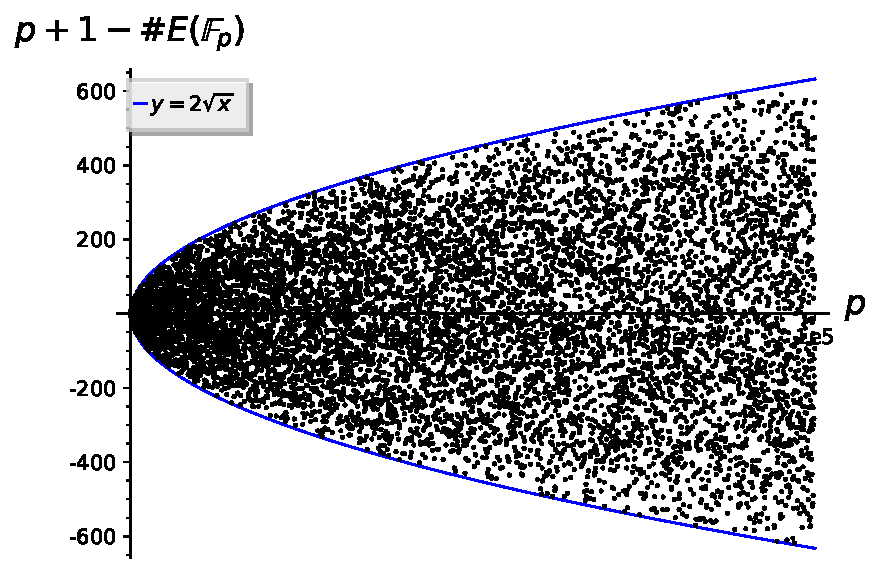
\includegraphics[width=.7\textwidth]{pointcounts.pdf}
\caption{Il·lustració del Teorema de Hasse per la corba $E\colon y^2=x^3-x+1$}
\end{figure}
\FloatBarrier
\end{example}
El que s'observa a la gràfica s'expressa en forma de teorema:
\begin{theorem}[Teorema de Hasse]
 Si $E$ és una corba el·líptica definida sobre $\F_q$, aleshores
 \[
 |\# E(\F_q) - (q+1)|\leq 2\sqrt{q}.
 \]
\end{theorem}
\begin{proof}[Idea de la demostració.]
Recordem la isogènia de Frobenius $\phi_E$. Observem que $E(\F_q)=\ker(\phi_E-1)$, i per tant ens interessa calcular $\#\ker(\phi_E-1)$. Aplicarem la desigualtat de Cauchy--Schwartz a $\varphi_1=\phi_E$ i $\varphi_2=[1]$. De la forma normal de $\phi_E$ veiem que $\deg(\phi_E)=q$. Per altra banda, resulta que $\deg(\phi_E-1)=\#\ker(\phi_E-1)$. Observem aleshores que $\#E(\F_q)=\#\ker(\phi_E-1)=\deg(\phi_E-1)$, i per tant obtenim directament el resultat.
\end{proof}

\begin{proposition}
 Sigui $E/\F_q$ una corba el·líptica. Aleshores $\phi_E$ satisfà
\[
\phi_E^2 - a\phi_E + q =0,\text{ on }\ a= q+1 - \#E(\F_q).
\]
\end{proposition}
\begin{proof}
 Considerem l'endomorfisme $f = \phi_E^2-a\phi_E+q$, que volem veure que és $0$. Com ja hem vist, $f$ indueix una aplicació lineal $f_m\in \End(E[m])$, per a tot $m\geq 1$. Si $m$ és coprimer amb $q$, aleshores $E[m]\cong (\Z/m\Z)^2$. Del fet que $\phi_E$ té grau $q$, que $\phi_E-1$ té grau $\#E(\F_q)$, i que $\det(\phi_m)) \equiv \deg(\phi)\pmod{m}$ en deduïm, evaluant el polinomi característic de $\phi_m$ a $1$, que $\operatorname{tr}(\phi_m) \equiv a \pmod{m}$. Per tant, $f_m\equiv 0\pmod{m}$, i això vol dir que el nucli de $f$ conté $E[m]$. Com que $m$ es pot fer arbitràriament gran, concloem que $f$ té nucli infinit. Per tant, $f=0$, com volíem veure.
\end{proof}
\begin{remark}
\label{remarca:frobenius}
La proposició diu que per a tot punt $P=(x,y) \in E(\bar\F_q)$, es té
\[
(x^{q^2},y^{q^2}) - a\cdot (x^q,y^q) + q\cdot(x,y) = \calO_E.
\]
\end{remark}

El següent teorema ens dona una manera fàcil de calcular $\#E(\F_{q^n})$ si la corba $E$ està definida sobre $\F_q$ i sabem calcular $\#E(\F_q)$. Per enunciar-lo, ens cal considerar les arrels $\alpha, \beta$ del polinomi $X^2-aX+q$, on $a=q+1-\#E(\F_q)$.

\begin{lemma}
Les arrels $\alpha$ i $\beta$ del polinomi $X^2-aX+q$ són o bé les dues iguals o bé complexos conjugats. En tot cas, satisfan $|\alpha|=|\beta|=\sqrt{q}$.
\end{lemma}
\begin{proof}
 Pel Teorema de Hasse, el polinomi $X^2-aX+q$ té discriminant $a^2-4q\leq 0$. Si aquest discriminant és $0$ (i per tant $q$ és un quadrat) aleshores $X^2-aX+q = (X\pm\sqrt{q})^2$. Si $a^2-4q<0$, aleshores $\alpha$ i $\beta$ són complexos conjugats i el seu producte és $q$. Per tant, tenim $|\alpha|=|\beta|=\sqrt{q}$.
\end{proof}
\begin{theorem}
 Sigui $E$ una corba el·líptica definida sobre $\F_q$. Aleshores,
 \[
 \# E(\F_{q^n}) = q^n + 1 - \alpha^n - \beta^n,\quad \forall n\geq 1.
 \]
\end{theorem}
\begin{proof}
Definim $s_i=\alpha^i+\beta^i$. Per altra banda, observem que el polinomi $X^{2i}-s_iX^i+q^i$ es pot escriure com $(X^i-\alpha^i)(X^i-\beta^i)$. Sabem que el primer factor és múltiple de $X-\alpha$ i el segon és múltiple de $X-\beta$ i, per tant, el polinomi $X^{2i}-s_iX^i+q^i$ és un múltiple de $X^2-aX+q$. Això implica que $\phi_E^n$ satisfà el polinomi $X^2-s_nX+q^n$. Si pensem ara en $E$ com una corba sobre $\F_{q^n}$ i apliquem la proposició anterior, obtenim que $\phi_E^n$ també satisfà $X^2-t_nX+q^n$, on $t_n=q^n+1-\#E(\F_{q^n})$. Per tant, satisfà la seva diferència, és a dir: $(t_n-s_n)\phi_E^n = 0$. Com que $\phi_E^n$ no és zero, n'extreiem que $s_n=t_n$, que és el que volíem veure.
\end{proof}
\begin{remark}
El teorema anterior ens dona una manera recursiva de calcular $\#E(\F_{q^n})$ sense treballar amb nombres complexos ni amb arrels quadrades. Si escrivim $s_i=\alpha^i+\beta^i$, observem que $s_0=2$ i $s_1=a$, i es demostra directament que
\[
s_{n+1}=\alpha^{n+1}+\beta^{n+1} = (\alpha+\beta)(\alpha^n+\beta^n) - \alpha\beta(\alpha^{n-1}+\beta^{n-1}) =
as_n-qs_{n-1}, \quad n\geq 2.
\]
\end{remark}

 \subsection{Criptografia amb corbes el·líptiques}
 
 \subsubsection{Diffie--Hellman amb corbes el·líptiques}
 Recordem que el protocol de Diffie--Hellman fa servir l'operació de grup a $\F_p^\times$, que és un grup cíclic, per establir una clau comuna entre Alice i Bob. Podem canviar el grup $\F_p^\times$ pel grup generat per un punt $P\in E(\F_q)$. Denotem per $N$ l'ordre del punt $P$ (fixem-nos que $N\simeq q$, pel teorema de Hasse). Això resulta en el següent protocol (compareu-lo amb la \S\ref{sec:diffie-hellman}).
 
 \begin{enumerate}
    \item L'Alice escull un enter a l'atzar $1<a<N$, i envia el punt $Q_A=aP\in E(\F_q)$ a en Bob.
    \item En Bob, per la seva banda, escull un enter a l'atzar $1<b<N$, i envia el punt $Q_B=bP\in E(\F_q)$ a l'Alice.
    \item L'Alice i en Bob calculen respectivament $aQ_B$ i $bQ_A$. Observem que els dos punts calculats són iguals a $abP$, que serà el secret compartit.
\end{enumerate}

En aquest cas, també es creu que \emph{problema de Diffie--Hellman per corbes el·líptiques (ECDHP)} i el \emph{problema del logaritme discret per corbes el·líptiques (ECDLP)} són equivalents. Òbviament, la seguretat del sistema depèn de l'ordre $N$ del punt $P$ escollit, i per tant ens interessarà trobar corbes el·líptiques $E/\F_q$ tals que $\#E(\F_q)$ sigui divisible per un primer gran.

Per altra banda, l'algoritme més potent per resoldre el logaritme discret a $\F_q^\times$, que s'anomena ``Index Calculus'', no té anàleg a $E(\F_q)$. Això fa que per solucionar el logaritme discret a $E(\F_q)$ només es tinguin disponibles els algoritmes que funcionen per grups cyclic genèrics. Conseqüentment, un sistema criptogràfic basat en l'ECDLP pugui assolir la mateixa seguretat que un sistema basat en el DLP treballant amb un cos finit de cardinal molt menor.

La companyia Certicom\footnote{\url{https://www.certicom.com/content/certicom/en/the-certicom-ecc-challenge.html}} té diferents reptes de resoldre el logaritme discret en corbes el·líptiques, i ofereix 20.000\$ a qui trobi el logaritme discret d'un punt concret d'una corba $E$ definida sobre $\F_p$, on $p=1550031797834347859248576414813139942411$ (131 bits). En canvi, des del 2005 es pot (amb tècniques molt avançades i amb molt d'esforç computacional) resoldre el logaritme discret per primers d'aquest tamany. De fet, es pot fer per primers de fins a 180 bits. Es considera que la seguretat en corbes el·líptiques obtinguda amb primers d'uns 160 bits és comprable a l'obtinguda a $\F_p^\times$ amb primers de 1024 bits, mentre que amb només 256 bits s'obté la seguretat corresponent a 4096 bits de $\F_p^\times$.

 \subsubsection{ElGamal amb corbes el·líptiques}
 El xifrat ElGamal també es pot dur a terme amb corbes el·líptiques. Aprofitarem per descriure l'algoritme per un grup $G=\F_q^\times$ o $G=E(\F_q)$. En el cas $G=\F_q^\times$ recuperaríem l'algoritme de la \S\ref{sec:elgamal}
 
 \begin{description}
 \item[Preparació: ] Cada usuari (posem Alice) tria un element $g\in G$ d'ordre $N$ suficientment gran. Seguidament, tria un enter $2< a < N$ i calcula $A=g^a$. La clau pública de l'Alice serà la tupla $(G,g,A)$, i la clau secreta serà $a$.
 \item[Xifrat: ] Suposem que en Bob vol enviar un missatge $m\in G$ a l'Alice. En Bob tria un enter a l'atzar, $2< y < N$, i calcula $Y=g^y\in G$ i també $Z=mA^y$. Aleshores envia a Alice la tupla $(Y,Z)$.
 \item[Desxifrat: ] Per recuperar el missatge, Alice calcula $Y^{-a} Z$. Observem que
 \[
 Y^{-a}Z = g^{-ay}mg^{ay} = m.
 \]
 \end{description}
 
 \subsection{Comptatge de punts: l'algoritme de Schoof}
 En aquest apartat volem estudiar el problema de determinar, donada una corba $E/\F_p$, el nombre de punts $\# E(\F_p)$. Ja sabem que, pel Teorema de Hasse,
 \[
 \# E(\F_p) = p + 1 - a,\quad\text{amb } |a|\leq 2\sqrt{p}.
 \]
 Suposem també que $p>3$ (en cas contrari, és molt fàcil determinar $E(\F_p)$), i escrivim $E$ en la forma $E\colon y^2=x^3+Ax+B$, amb $A,B\in\F_p$.
 Per cada $x\in \F_p$, definim
 \[
 \chi(x)=\begin{cases}
 0&\text{si } x=0,\\
 +1&\text{si } x\in(\F_p^\times)^2,\\
 -1&\text{si } x\in \F_p^\times\smallsetminus (\F_p^\times)^2.
 \end{cases}
 \]
 Aleshores, observem que
 \[
 \# E(\F_p) = 1+ \sum_{x\in\F_p} (1+\chi(x^3+Ax+B))= 1+p+\sum_{x\in\F_p} \chi(x^3+Ax+B),
 \]
 i per tant tenim una formula tancada per $a$:
 \[
 a = -\sum_{x\in\F_p}\chi(x^3+Ax+B).
 \]
 Més endavant veurem una manera eficient de calcular $\chi(x)$ per qualsevol $x\in\F_p$. Tot i així, si $p$ és molt gran (que sigui útil en criptografia) no podrem recórrer\footnote{En l'actualitat es fan servir primeres d'entre $50$ i $80$ xifres decimals, i cal tenir en compte que un ordinador actual trigaria l'edat de l'univers a recórrer els enters entre $1$ i $10^{27}$.} tots els elements de $\F_p$.
 
 El 1985, R.~Schoof va donar el primer algoritme que calculava $\#E(\F_p)$ amb un nombre d'operacions polinomial en $\log(p)$, fet que va permetre d'utilitzar les corbes el·líptiques en la criptografia de manera pràctica. Seguidament veurem les idees principals de l'algoritme d'Schoof.
 
 A la Remarca~\ref{remarca:frobenius} hem vist que si $P=(x,y)\in E(K)$, on $K/\F_p$ és una extensió qualsevol, aleshores
 \begin{align}
 \label{eq:frobenius-schoof}
 (x^{p^2},y^{p^2}) + [p] (x,y) = [a] (x^p,y^p).
 \end{align}
 La quantitat de l'esquerra es pot calcular de manera eficient, fent servir exponenciació modular pel primer terme, i l'anàleg de l'exponenciació modular per corbes el·líptiques pel segon.
 
 \begin{remark}
 Fixem-nos que l'enter $a$ no es pot extreure directament de $[a]$ actuant en punt qualsevol, ja que si $(x,y)$ té ordre $N$, aleshores $(x^p,y^p)$ també (per què?), i per tant $[a+kN](x^p,y^p)=[a](x^p,y^p)$ per a tot $k$. Així, el punt $(x,y)$ només permet determinar $a$ mòdul $N$. 
 \end{remark}
 
 La idea de Schoof consisteix en determinar $a\pmod \ell$ per suficients primers $\ell$ petits, i després reconstruir $a$ fent servir el teorema xinès dels residus. Per exemple, per determinar $\#E(\F_p)$ amb $p\simeq 10^{71}$ n'hi ha prou amb considerar $2<\ell<100$. Afegint-hi els 5 primers que hi ha fins a $\ell < 115$ ja podem determinar $\#E(\F_p)$ amb $p\simeq 10^{91}$, i amb dos primers més ($127$, $131$) ja podem arribar a $p\simeq 10^{100}$.

 Fem primer el cas $\ell=2$.
 \begin{lemma}
 L'enter $a$ és parell si, i només si, $x^3+Ax+B$ té arrels a $\F_p$.
 \end{lemma}
\begin{proof}
 Recordem que $x^3+Ax+B$ factoritza a $\F_p$ si i només si $E(\F_p)$ té un element d'ordre $2$, que serà de la forma $(\alpha,0)$ on $\alpha$ és una arrel de $x^3+Ax+B$. Ara bé, com que $p$ és senar tenim
 \[
 \# E(\F_p) = p+1-a\equiv a\pmod 2,
 \]
 i $E(\F_p)$ té un element d'ordre $2$ si i només si $\#E(\F_p)$ és parell.
 \end{proof}
 
 Així, considerem ara un primer $\ell$ senar, i ens cal trobar un punt d'ordre $\ell$. No podem esperar que aquest punt estigui definit a $\F_p$, i per tant en general haurem de considerar extensions $K/\F_p$. 
 
 \begin{theorem}
 \label{thm:division-polys}
  Considerem els polinomis $\psi_m\in\Z[x,y]$,
  \begin{align*}
  &\psi_1=1,\quad \psi_2=2y,\quad \psi_3 = 3x^4+6Ax^2+12Bx-A^2,\\
  &\psi_4=4y(x^6+5Ax^4+20Bx^3-5A^2x^2-4ABx-8B^2-A^3),\\
  &\psi_{2m+1}=\psi_{m+2}\psi_{m}^3 - \psi_{m-1}\psi_{m+1}^3,& (m\geq 2),\\
  &\psi_{2m}=\frac{\psi_m}{2y}(\psi_{m+2}\psi_{m-1}^2-\psi_{m-2}\psi_{m+1}^2),& (m\geq 3).
  \end{align*}
  Aleshores per a tot primer senar $\ell\neq p$, es té $\psi_\ell \pmod p \in \F_p[x,y^2]$ i, si substituim $y^2=x^3+Ax+B$ obtenim un polinomi en $x$ de grau $\frac{\ell^2-1}{2}$. A més, $P\in E(\bar\F_p)[\ell]\smallsetminus\{\calO\}\iff \psi_\ell(x(P))=0$.
 \end{theorem}
 \begin{corollary}
 Per tot primer $\ell\neq p$, es té $E[\ell]\cong\Z/\ell\Z\oplus\Z/\ell\Z$.
 \end{corollary}
 \begin{proof}
  Els punts d'$E[\ell]=E(\bar\F_p)[\ell]$ són de la forma $(\alpha, \beta)$ on $\alpha$ és una arrel de $\psi_\ell$. Per tant, $\# E[\ell]=1+2\deg(\psi_\ell)=\ell^2$. Com que tot $E[\ell]$ té exponent $\ell$,  necessàriament $E[\ell]=(\Z/\ell\Z)^2$.
 \end{proof}
 Si prenem $K/\F_p$ un cos on $\psi_\ell$ tingui alguna arrel $\alpha$, aleshores podem considerar el punt de $\ell$-torsió $P=(\alpha,\sqrt{D})\in E(K(\sqrt{D}))$, on $D=\alpha^3+A\alpha+B$. Per tant, per determinar $a\bmod \ell$ caldrà calcular múltiples de $P$ en el grup $E[\ell](K(\sqrt{D}))$. Fixem-nos que aquest cos té un grau gran ($\ell^2-1$), i per tant les operacions seran molt costoses si $\ell$ es fa moderadament gran.
 
 Podem treballar al cos $K$, sense afegir una arrel de $D$: considerem la corba
 \[
 E^D \colon y^2 = x^3 + AD^2x + BD^3.
 \]
 Aleshores, si escrivim $\delta=\sqrt{D}$, tenim un isomorfisme $\tau\colon E\to E^D$ que envia $(x,y)$ a $\tau(x,y)=(Dx,\delta^3y)$, i que ens permet realitzar totes les operacions a $E^D(K)$. Fixem-nos que si $D$ és un quadrat, aleshores $E$ és isomorfa a $E$ (via $\tau$) però en general l'isomorfisme està definit sobre una extensió de grau $2$. En tot cas, observem que
\begin{align*}
    \tau((\alpha,\delta)) &= (D\alpha, D^2),\quad \tau((\alpha^p,\delta^p))=(D\alpha^p,D^{\frac{p+3}{2}}),\quad
    \tau((\alpha^{p^2},\delta^{p^2})) =(D\alpha^{p^2},D^{\frac{p^2+3}{2}}).
\end{align*}
Per tant, l'equació~\eqref{eq:frobenius-schoof} és equivalent a la següent equació a $E^D$:
\[
(D\alpha^{p^2},D^{\frac{p^2+3}{2}}) + [p] (D\alpha,D^2) = [a] (D\alpha^p,D^{\frac{p+3}{2}}).
\]


Acabem la secció amb una implementació en  \texttt{Sage} de l'algoritme d'Schoof.

\begin{algo}
   \caption{Donats $E$ i un primer $p$, calcula $p+1-\#E(\F_p)$.}
\begin{python}    
def t_mod(A, B, p, ell):
    pmod = p % ell
    if pmod > ell / 2:
        pmod -= ell
    A = GF(p)(A)
    B = GF(p)(B)
    t = PolynomialRing(GF(p), 't').gen()
    if ell == 2:
        return 1 if (t^3+A*t+B).is_irreducible() else 0
    E0 = EllipticCurve([0,0,0,A,B])
    h = E0.division_polynomial(ell,t,0).factor()[0][0]
    K.<r> = FiniteField(p^h.degree(), modulus = h)    # K = F[x]/(h(x))
    D = r^3 + A * r + B
    E = EllipticCurve([A*D^2, B*D^3])
    P = E([D*r, D^2])
    phi_P = E([D * r^p, D^((p+3)//2)])
    phi2_P = E([D * r^(p^2), D^((p^2+3)//2)])
    LHS = phi2_P + pmod * P; RHS = E(0)
    for a in range((ell+1) // 2):
        if LHS ==  RHS: return a
        elif LHS == -RHS: return -a
        RHS += phi_P
\end{python}

\begin{python}
def Schoof(A, B, p): # y^2 = x^3 + Ax + B 
    M = 1; ell = 1; S = []; traces = []
    while M <= 4*RR(p).sqrt():
        ell = next_prime(ell); S.append(ell); M *= ell
        traces.append(t_mod(A, B, p, ell))      
    a = CRT(traces, S) # Fem servir el Teorema Xinès dels Residus
    return a if a < M / 2 else a - M
  \end{python}
\end{algo}


Finalment, vegem la complexitat d'aquest algoritme. Els polinomis $\psi_\ell$ tenen grau $O(\ell^2)=O(\log^2 p)$. Per tant, els elements de l'extensió $K$ tenen tamany $O(\ell^2\log p)=O(\log^3 p)$. Per calcular $\alpha^p$ i $\alpha^{p^2}$ calen $O(\log p)$ operacions a $K$, i per tant en total $O((\log p)(\log^3 p)^2)$, és a dir $O(\log^7 p)$. Com que això s'ha de fer per $O(\log p)$ primers (pel Teorema dels Nombres Primers), en total calen $O(\log^8 p)$ operacions de bit. Si es poden fer operacions a $K$ de manera més ràpida (per exemple fent servir transformades de Fourier) es pot reduir la complexitat a $O(\log^{5+\epsilon} p)$. Millores posteriors de Elkies i Atkin permeten calcular $\#E(\F_p)$ amb temps $O(\log^{4+\epsilon} p)$.